\documentclass[ExampleMasters.tex]{subfiles}

\tikzstyle{wide} = [rectangle, rounded corners, minimum width=1cm, minimum height=1cm,text centered, draw=black]
\tikzstyle{narrow} = [rectangle, rounded corners, minimum width=0.5cm, minimum height=1cm,text centered, draw=black]
\tikzstyle{narrow1} = [rectangle, rounded corners, minimum width=0.5cm, minimum height=1cm,text width = 3cm, text centered, draw=black]
\tikzstyle{arrow} = [thick,->,>=stealth]

\begin{document}

\chapter{Mission Productivity}

	\section{Introduction}
		The addition of electric propulsion on axles other than the conventional engine-propelled axles in long combinations is necessary to meet power and gradeability requirements as well as the performance based standards. The choice of axles is to be well-motivated and quantifiable. An objective numerical standard of comparison between different combinations and propulsion configurations for specific missions can thus be provided by the mission productivity factor. The objective function used to represent mission productivity will be sought to be maximised. In the following sections, various definitions of mission productivity in the heavy truck transport context will be presented. The definition chosen to be optimised will then be formulated and discussed in detail. 

	\section{Mission productivity definitions}
		Productivity is expressed as the number of units of output that a given number of units of input / investment yields. OECD defines productivity as "the ratio of a volume measure of output to a volume measure of input"\cite{OECDProd}. The outputs of a production or transport process are often influenced by a combination of several factors or 'inputs', that may themselves be dependent on one another. Depending on the nature and quantity of reference inputs against which productivity is measured, the latter can be classified as follows \cite{JapSNAOECD}:

		\begin{itemize}
			\item \textbf{Single factor productivity} - The outputs of a process are often measured relative to a single input either due to its relative importance among all possible factors or to observe the individual trends of output performance specific to the input chosen. For example, labour or workforce productivity measures the volume output relative to the number of working hours spent by an employee \cite{TruckProdAus, WikiLabourProd}. In the current perspective, the mission productivity relative to a single factor such as driver expenses or fuel consumption is an example of such a measure.

			\item \textbf{Multi-factor productivity} - When the influences of several individual inputs to a system or process are considered inseperable, the productivity measure is defined relative to a combination of all the inputs expressed suitably as an expression. For example, the Gross Domestic Product is a productivity measure relative to a host of factors such as population, economy and education among several others \cite{TruckProdAus, WikiGDP}. In the current context, mission productivity can be expressed with respect to a combination of factors such as fuel economy, electricity prices, driver costs, maintenance costs and fixed purchasing costs. 
		\end{itemize}

		The productivity measure for a heavy truck-trailer combination serves as a fitness measure to evaluate the economic and environmental viability of the combination on a given specific mission. It can be deduced from the above that the fitness measure is hence mission dependent and is thus bound to vary depending on the route chosen, type of payload carried, number of starts and stops and driver behaviour among several other mission parameters. Thus, it can inferred that the productivity measure, when optimised for each mission, will yield different optimal combinations suited for the mission at hand.\\

		A few different mission productivity measures are briefly considered below:
		\begin{itemize}
			\item \textit{Load per vehicle kilometre} - This single factor productivity measure, P1, focuses on the quantity of payload transported for every kilometre of vehicle distance covered and can thus be optimised by reducing mission time to increase number of annual trips, increase axle load capacities and improving average combination speeds while preserving key performance characteristics such as gradeability. These can be achieved by employing an improved powertrain or increased axle propulsion. The measure does not consider fuel consumption, fixed costs etc. though.

			\begin{equation}
				P1 = \frac{M_{payload}*N_{trips}}{D_{annual}} \ tons/km
			\end{equation}

			where $N_{trips}$ is the average annual number of trips covered for the given mission, $M_{payload}$ is the average load carried per mission (kg) and $D_{annual}$ is the average total vehicle distance covered (km).

			\item \textit{Annual freight per vehicle} - This measure, P2, is indicative of the utilisation of the vehicle and is expressed in number of tonne-kilometres covered annually \cite{TruckProdAus}. Thus, the number of useful transportation kilometres coupled with the quantity of payload transported forms the basis for the measure. This too, does not consider fuel consumption and other mission outputs.

			\begin{equation}
				P2 = M_{payload}*D_{annual} \ tonne-km
			\end{equation}

			\item \textit{Average operating costs per vehicle kilometre or freight transported} - The operating costs involve fuel consumption, driver expenses and maintenance costs and are sought to be minimised against every unit tonne-kilometre freight. While this measure, P3, is a more meaningful quantity, it fails to adequately address the business profitability of ownership and transport.

			\begin{equation}
				P3 = \frac{Cost_{operating}}{M_{payload}*D_{annual}},\ or\ \frac{Cost_{operating}}{D_{annual}} \  \euro/tonne-km \ or \ \euro/km 
			\end{equation}

			where $Cost_{operating}$ is the average annual operating cost. This may itself be expressed as 

			\begin{equation}
				Cost_{operating} = Cost_{fuel} + Cost_{personnel} + Cost_{maintenance} + Cost_{miscellaneous} \ \euro
			\end{equation}

			where $Cost_{fuel}$ is the average annual fuel expense, $Cost_{personnel}$ is the average annual cost incurred by employment of personnel including the driver, $Cost_{maintenance}$  is the average annual cost of maintenance of the truck and associated operational elements and $Cost_{miscellaneous}$ is the sum of all miscellaneous costs arising from the freight transport.\\

			\item \textit{Freight per driver hour} - In developed economies, personnel costs in heavy trucking can account for upto 44\% in long haul operations. The dominant contribution of personnel expenses to transportation costs thus implies that the freight transport productivity relative to investment in drivers and other personnel, P4, must be maximised. This, of course, must not be achieved at the expense of high fuel prices resulting from aggressive driving to minimise mission times. 

			\begin{equation}
				P4 = \frac{M_{payload}*D_{annual}}{T_{driver}} \ tonne-km/hour
			\end{equation}

			where $T_{driver}$ is the average annual number of driver hours billed to the freight transport company (including rest and halt hours).\\

			\item \textit{Freight per unit fuel consumed} - The ratio of driver to fuel expenses is reversed in developing economies where fuel prices can account for upto 45\% of the transportation costs. Here, maximising the freight transport per litre of fuel consumed, P5, becomes more pertinent.
			
			\begin{equation}
				P5 = \frac{M_{payload}*D_{annual}}{V_{fuel}} \ tonne-km/litre
			\end{equation}

			where $V_{fuel}$ is the average annual fuel consumption in litres.\\

			\item \textit{Emissions per unit freight transported} - The environmental impact of freight transport can be quantified in terms of the number of milligrams of carbon dioxide emissions generated per tonne-kilometre of freight transported, P6. This become relevant especially in the current context where additional electric propulsion can improve not only vehicle gradeability and average speed, but also reduce vehicle emissions. The combination that has the least carbon footprint for the given mission can thus be identified and the transportation expenses viewed more holistically. The fixed costs in the optimisation schedule will thus vary depending on the exhaust after-treatment systems used; maintenance costs will depend on the quantity of AdBlue used, number of diesel particulate filters replaced etc.

			\begin{equation}
				P6 = \frac{M_{emissions}}{M_{payload}*D_{annual}}\  mg/tonne-km
			\end{equation}

			where $M_{emissions}$ is the average annual number of milligrams of carbon dioxide and other noxious pollutant emissions generated by the vehicle.

			\item \textit{Revenue earned per unit investment} - From the logistics provider's perspective, the maximisation of returns on investment, or profit maximisation, over a fixed number of years is primal. This depends not only on the freight transported, driver, fuel and maintenance expenses and fixed initial costs, but also on the type of payload being transported and the revenue earned from each mission. This measure, P7, is thus a multi-factor productivity factor that is sensitive to several input factors as mentioned above.

			\begin{equation}
				P7 = \frac{Revenue_{annual}*N_{first\ owner}}{Cost_{fixed} + Cost_{variable}}\ \euro/\euro
			\end{equation}

			where $Revenue_{annual}$ is the average annual revenue earned over a target duration of $N_{first\ owner}$ years, $Cost_{fixed}$ is the initial investment in the tractor, trailers and machinery and $Cost_{variable}$ is the total operating cost over $N_{first\ owner}$ years.

		\end{itemize}

		While single factor productivity measures such as fuel costs per kilometre travelled are valid figures, their relevance can be skewed when viewed in a wider perspective. For example, as shown in Table \ref{table:fuelConsumptionRate} \cite[T.~2.8]{TruckProdAus}, the average fuel consumption per kilometre travelled for articulated trucks increased from 45.7 to 49.5 litres per 100 kilometres during the years 1971 and 2007. During the same period of time, in comparison, the fuel consumption per unit freight (tonne-kilometre) dropped by 44\% from 4.7 to 2.7 litres per 100 ton-kilometres \cite{TruckProdAus}. Hence, the choice of productivity measure is key to arriving at the right objective function to optimise.\\

		\begin{table}[ht]
			\centering 
			\begin{tabular}{l c c c c}
  			\hline
			Vehicle type & \multicolumn{4}{c}{Fuel consumption rate}\\ \cline{2-3} \cline{4-5}
			\ & \multicolumn{2}{c}{Per VKT} & \multicolumn{2}{c}{Per TKM}\\ \cline{2-3} \cline{4-5}
			\ & 1971 & 2007 & 1971 & 2007\\ \hline
			    LCVs  & 12.8 & 12.8 & 108.7 & 60.7\\
			    Rigid trucks  & 23.3 & 26.0 & 12.7  & 7.2\\
			    Articulated trucks  & 45.7 & 49.5 & 4.7 & 2.7  \\
			    All CVs  & 27.9 & 36.4 & 8.1 & 3.5 \\
			    All HVs  & 19.9 & 19.8 & 11.8 & 6.2 \\
			\hline 
			\end{tabular}
			\caption{Fuel consumption per freight tonne kilometre, 1971-2007 \cite{TruckProdAus}} 
			\label{table:fuelConsumptionRate} 
		\end{table}

		Since profit maximisation of transport customers is the object of prime focus while choosing freight transport configurations, it can be agreed that the corresponding productivity measure is a multi-factor one, depending on a number of input parameters as explained in the forthcoming section.\\

	\section{Productivity measure - Choice and Definition}

	The goals sought to be achieved by the European Modular Systems as set out by the EMS Internal Platform Group are as follows \cite{EMSleaflet}:
	\begin{itemize}
		\item Meeting growing freight transport demands
		\item Reducing fuel consumption
		\item Reducing emissions
		\item Reducing operating costs for freight transporters
	\end{itemize}

	\begin{figure}[h!]
		\centering
		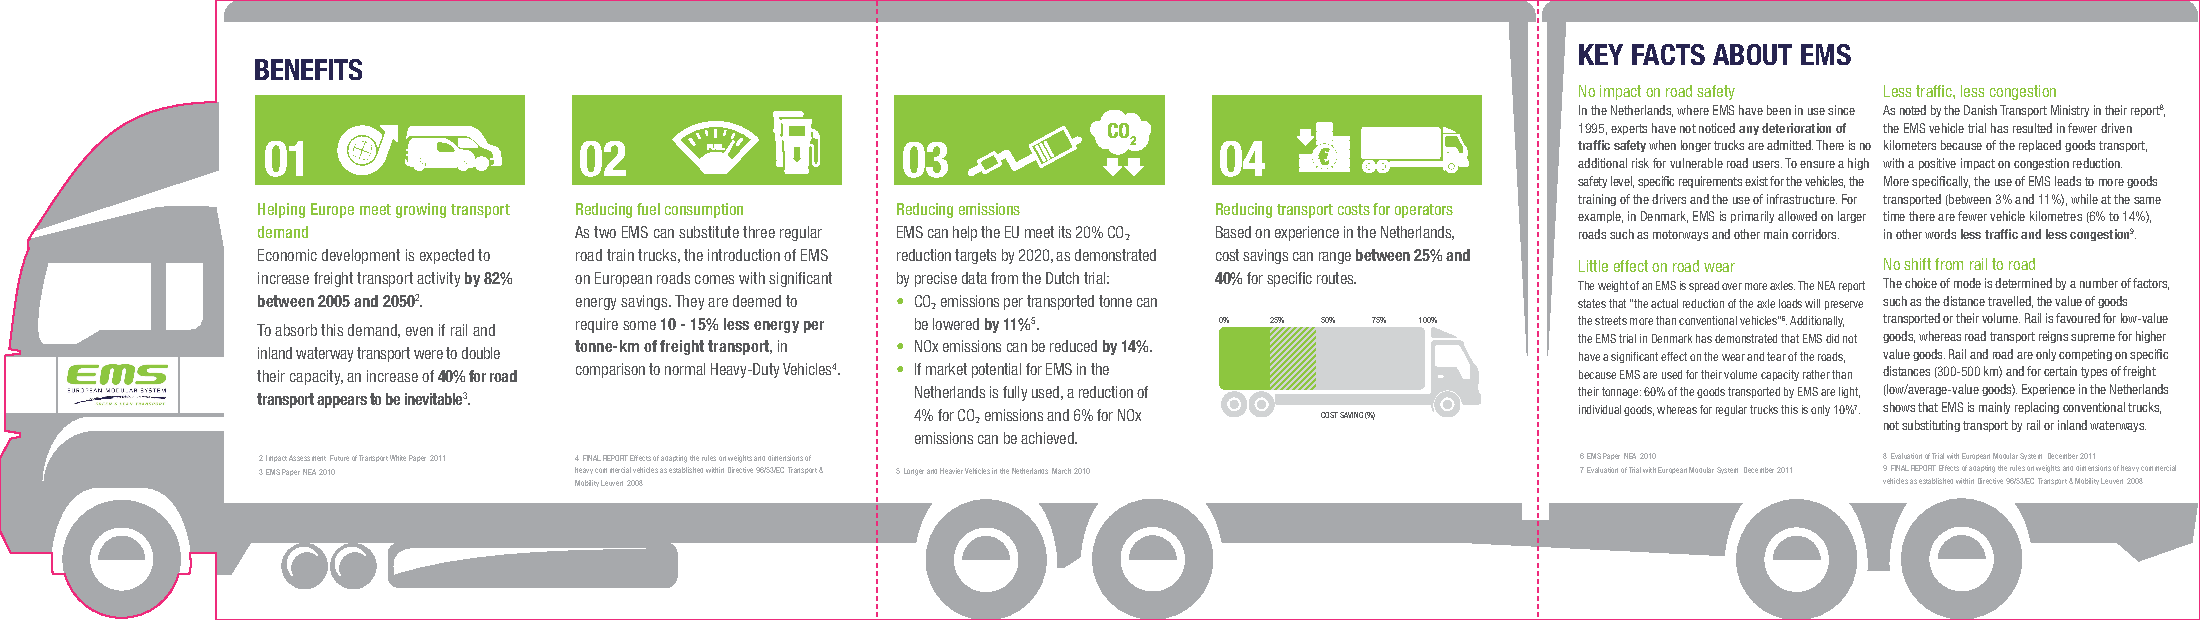
\includegraphics[width=\linewidth, clip=true, trim=0 0 325 0]{figures/eea_leaflet.pdf}
		\caption{Goals of the European Modular System \cite{EMSleaflet}}
		\label{EMSleaflet}
	\end{figure}

	It can hence been seen that, seen from the freight transporter's prespective, the productivity measure must focus on maximising freight carried while capping fuel consumption and associated emissions, while still producing revenues that promote profit maximisation. Thus, the last productivity measure defined in the previous section, revenue earned per unit investment, is chosen as a reasonable complete measure that incorporates the salient goals of the EMS.\\ 

	The productivity factor, P, is redefined below for clarity:
	\begin{equation}
		P = \frac{Revenue_{annual}*N_{first\ owner}}{Cost_{fixed} + Cost_{variable}}\ \euro/\euro
	\end{equation}

	where $Revenue_{annual}$ is the average annual revenue earned over a target duration of $N_{first\ owner}$ years, $Cost_{fixed}$ is the initial investment in the tractor, trailers and machinery and $Cost_{variable}$ is the total operating cost over $N_{first\ owner}$ years.\\

	$Revenue_{annual}$ is usually defined in terms of the average gross transporter income or gross transport costs per unit freight transported, per vehicle kilometer. It can be gleaned from literature that the former definition is known to vary between 4 and 6 US Dollar Cents per tonne-kilometre \cite{WorldBankReport} while the latter is in the range of 0.75 USD per kilometre to 1.25 USD per kilometre \cite{WorldBankReport}.\\

	The initial buying prices of trucks, trailers, additional loading equipment and superstructures form the bulk of the fixed costs, $Cost_{fixed}$. Average truck prices in the context of the European buyer are considered in this thesis, with a step-up margin for the three different powertrain sizes considered in the optimisation tool. It must be noted though, that the axle load configurations, cab specifications and other truck parameters have a significant bearing on actual buying prices, aside from taxation policies and registration schedules that vary internationally. Frost \& Sullivan \cite{FrostSullivan} estimates average upfront truck prices ranging between 110,000 USD and 125,000 USD and trailer prices ranging between 30,000 USD and 50,000 USD for the year 2014. This thesis places the dolly and semitrailer prices at the lower and upper bounds for the trailer prices respectively. The truck price is assigned to the base powertrain configuration and premiums of x\% and y\% are assigned to the higher powertrain configurations respectively, based on Volvo's Cost-Calc tool.\\

	In this thesis, the price of electrified axles is incorporated in the form of add-on features and are thus simple additive terms to the base price of the trailer. The electrification charges are divided primarily among the batteries, the electric machine and the auxiliary power electronics and control systems. Additionally, the additional mass of the electrification components is penalised by an appropriate reduction in payload tonnage capacity.\\

	Advances in battery technology are rapid and are expected to yield significant cost advantages over the years. Hence, a price trend analysis is necessary to evaluate how mission productivities can be maximised by the availability of cheaper batteries with higher energy densities in the decades to come. Lithium-ion batteries for plug-in hybrid vehicles with energy capacities in the range of 15-21 kWh are priced between 800 and 1200 \euro per kilowatt-hour today \cite{EUROBAT} and are expected to fall to 450 \euro per kilowatt-hour in the next decade \cite{EUROBAT}. The long-term trends predicted and published in \cite[T.~8-16]{ElementEnergy} are referenced for evaluations in productivity sensitivity to battery prices and are as shown in Table \ref{table:batteryPriceMassTrend}.\\

	DC electric motors rated between 75kW and 350kW are found to be priced approximately 29900 EUR \cite{EuPLot30Motors}.

	Variable costs or operational costs were estimated at approximately 80 EUR per hour for France and Germany \cite{EuAECOM}.

	\begin{table}[ht]
		\centering 
		\begin{tabular}{l c c c c c}
			\cline{2-6}
			\ & 2011 & 2015 & 2020 & 2025 & 2030\\ 
			\hline
		    Pack cost (USD/kWh)  & 746 & 436 & 275 & 244 & 230\\
		    Pack mass (kg)  & 343 & 253 & 195  & 177 & 176\\
			\hline 
		\end{tabular}
		\caption{Battery price and mass trends 2011-2030 \cite{ElementEnergy}} 
		\label{table:batteryPriceMassTrend} 
	\end{table}

	\section{Design variable definition}
		The choice of design variables and design parameters must be made before the objective formulation is taken up. Design variables are here defined as those configuration features that will be evaluated and determined as a result of the optimisation runs. Design parameters are defined as those configuration features that closely influence the productivity function but remain constant for a chosen population. With this distinction set up, the design variables can be briefly as listed below. It must be noted that the list is not exhaustive at the time of writing this report.

		\begin{itemize}
		\item Number of axles to be propelled in the combination (excluding the tractor axles)
		\item Motor sizing to match required tractive force
		\item Total size of energy buffers required
		\item Size of energy buffers for each trailing unit
		\item Differential sizing
		\end{itemize}

		The design parameters currently identified are listed below:

		\begin{itemize}
		\item Choice between in-wheel / single motor propelled axles
		\item Choice of energy management algorithm (EMA)
		\item Choice of conventional engine model (D11 / D13 / D16)
		\item Choice of hub-motors versus differential-driven trailer axles
		\item Battery and motor prices
		\item Fuel price
		\item Battery performance type in terms of end-of-lifetime State of Health ($\Delta SoH^{econ}$)
		\item Average yearly mileage for given combination / average number of trips per year
		\item Mission - route and speed profiles
		\item Type of payload and cost of transportation per kilometre per ton ( or per unit volume)
		\item Driver costs
		\item Yearly maintenance costs
		\item Markup percentage (?)
		\item Electricity price per kWh and fixed cost of setting up charging stations in case of plugins
		\end{itemize}

		It must be noted that the energy management algorithm may itself be set up as an individual sub-optimisation schedule with individual design variables and parameters.

	\section{Productivity definition}

		The productivity has been defined as a simple function of the costs and revenues as follows:\\

		\begin{equation}
			Productivity = \frac{Mission Revenue}{Mission Cost}
		\end{equation}

		As can be seen, the productivity is desired to be as large as possible. There are several components that contribute to the mission cost. Each of these have a fixed and variable / operating component. They are seperately described below:\\

		\subsection{Base combination cost}

			The combination without the electric axles consists of the tractor unit, dolly, B-semitrailer and the semitrailer. 

			\begin{equation}
				P_{tractor} = P_{chassis}+P_{engine}+P_{transmission}+P_{RAT}  (\euro{})\\
			\end{equation}
			\begin{equation}
				P_{tractor}^{purch}= markup*P_{tractor} (\euro{})\\
			\end{equation}
			\begin{equation}
				Cost_{combination}^{purch} = P_{tractor}^{purch}+P_{dolly}+P_{BST}+P_{ST} (\euro{})\\
			\end{equation}

			The mission operating cost due to just the combination can be written as 
			\begin{equation}
				Cost_{combination}^{operating} = annuit(Cost_{combination}^{purch}) (\euro{})
			\end{equation}

			We now elaborate the costs due to electrification of additional axles.

		\subsection{Batteries / Buffers}

			The buffer cost is best expressed in terms of cost per kWh of energy stored in the buffers. The buffer size is a design variable and the cost can be simply expressed as:

			\begin{equation}
				P_{battery}= Size_{buffer} \times Price_{perkWh} (\euro{})
			\end{equation}

			\begin{equation} 
				P^{purch}_{battery} = markup \times P_{battery} (\euro{})
			\end{equation}

			The total fixed cost of the buffers including maintenance is:

			\begin{equation} \label{8}
				Cost_{Battery}^{Fixed} = \frac{annuit(P_{battery})}{L_{mission}} (\euro{}/km)
			\end{equation}

			\begin{equation}
				\mu_{battery-replacement}^{mission} = \mu_{battery-replacement}^{econ} \times \frac{L_ {mission}}{L_{econ}} (units)
			\end{equation}

			where,
			\begin{equation}
				\mu_{battery-replacement}^{econ} = floor(\Delta SoH^{econ}\times \frac{L_ {mission}}{L_{econ}}) \times \frac{L_ {econ}}{L_{mission}} (units)
			\end{equation}

			The end-of-economic-lifetime state of health $\Delta SoH^{econ}$ and total lifetime distance $L_{mission}$ are design parameters. The motivation for these are drawn from [2]. Thus, the battery operating cost can be expressed as
			\begin{equation} \label{11}
				Cost_{Battery}^{Operating} = Cost_{Battery}^{Fixed} \times \mu_{battery-replacement}^{mission} (\euro{}/km)
			\end{equation}

			Thus, \eqref{8} and \eqref{11} together represent battery costs that add to the total cost in the productivity function:

			\begin{equation}
				Cost_{Battery} = Cost_{Battery}^{Fixed} + Cost_{Battery}^{Operating} (\euro{}/km)
			\end{equation}

		\subsection{Electric transmission}

			Since the motors can be said to transfer power from the energy buffers to the wheels, the total power rating of all the motors put together may not exceed that of the buffers. The choice of hub-motors (in-wheel motors) naturally suits torque vectoring in order to improve the lateral (yaw) performance of individual units. The more economical installation of a single motor coupled with a differential and drive shafts is also evaluated in this model through a switch choice. 

			The cost function for the electric drive is thus written as:

			\begin{equation}
				Cost_{electric-drive}^{fixed} = \frac{annuit(markup \times P_{electric-powertrain})}{L_{mission}} (\euro{}/km)
			\end{equation}
			where,
			\begin{equation}
				P_{electric-powertrain} = (n_{electric-machine} \times P_{electric-machine}) + (n_{mechanical-drives} \times P_{mechanical-drives}) (\euro{})
			\end{equation}

			\begin{equation}
				P_{electric-machine} = P_{electric-motor}+P_{auxiliary-equipment} (\euro{)}
			\end{equation}

			and,
			\begin{equation}
				P_{mechanical-drives} = P_{differential}+P_{drive-shafts} (\euro{})
			\end{equation}

			The auxiliary equipment comprises the power electronics, cooling and other supporting features associated with each motor installation. One does not expect to replace motors during the operating lifetime of the truck-trailer combination. Hence, the operating cost of the electric powertrain is owed to maintenance costs alone.

		\subsection{Fuel and electricity}
			Depending on if the combination is a pure hybrid or a plugin, the fuel costs associated with the combination can be differently calculated. This can be incorporated by means a of characterising design variable.

			\begin{equation}
				P_{fuel} = P_{fuel}^{mission}+P_{fuel}^{recharge} (\euro{})
			\end{equation}

			where,
			\begin{equation}
				P_{fuel}^{mission} = Mass_{fuel}^{mission} \times P_{fuel} (\euro{})
			\end{equation}

			and,
			\begin{equation}
				P_{fuel}^{recharge} = E_{recharge} \times P_{electricity, specific} (\euro{})
			\end{equation}

			In the above equations, $Mass_{fuel}^{mission}$ is obtained from the engine / energy management algorithm (EMA) combination as an output for the given mission.

		\subsection{Mass and time penalties}

			\begin{equation} \label{eq:time}
				Time bonus = (\Delta T \times P_{time-bonus}) (\euro{)}
			\end{equation}

			where,
			\begin{equation}
				\Delta T = \Delta T_{mission}+\Delta T_{charging} (hours)
			\end{equation}

			Costs incurred due to time spent in charging the vehicle must be included as downtime costs and find a place in the $\Delta T$ component in equation ~\ref{eq:time}. $\Delta T_{mission}$ refers to the reduction in mission time compared to the standard A-Double configuration. Here, $P_{payload-given-mission}$ refers to the returns in \euro{} per ton of payload being carried for the given mission. 

		\subsection{Reduction in conventional powertrain cost}
			The addition of electric propulsion provides the customer the opportunity to choose a lower engine specification at the cost of the electric machine. The goal, of course, remains to motivate this decision and validate the investment to be profitable. Based on the vehicle simulations, if it is found that the engine can be replaced with a lower horsepower one, the reduction in base price of the engine must reflect as a subtraction in the total cost.

			\begin{equation}
				Cost_{engine-downsizing} = -\Delta P_{engine,base-engine} (\euro{})
			\end{equation}

		\subsection{Driver Costs}
			The driver costs can be simply expressed in terms of the mission time and hourly rates as:

			\begin{equation}
			Driver-costs = Time_{mission} * Hourly_rates (\euro{})
			\end{equation}

		\subsection{Revenues}
			The revenues of the customer can be expressed simply as
			\begin{equation}
			Revenue = Mass_{payload} \times Earnings_{per-ton} (\euro{})
			\end{equation}

	\section{Simulation schedule}
		Several combinations of propulsion choices can be made for the given A-Double combination. Each of these must be evaluated for productivity in the optimisation algorithm. This is done by constructing a virtual vehicle model that corresponds to the configuration chosen for evaluation and simulating the vehicle for the chosen mission (road and load). The outputs of the simulation are fuel consumption, electricity usage, time taken apart from vehicle performance characteristics. The optimisation schedule takes fixed performance characteristics as constraints and uses these to eliminate unsafe or ill-performing combinations from the population.\\

		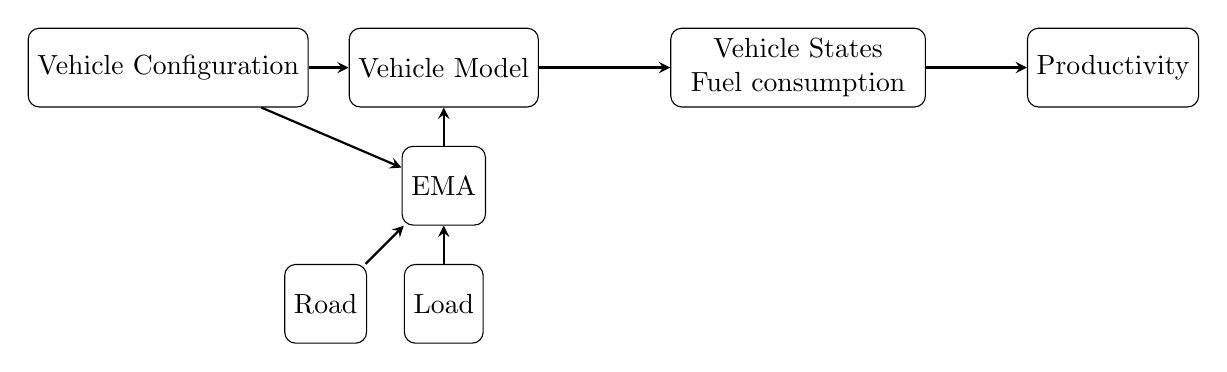
\begin{tikzpicture}[node distance=1.5cm]

		\node (conf) [wide] {Vehicle Configuration};
		\node (vmod) [wide, right of= conf, xshift=2cm] {Vehicle Model};
		\node (stat) [narrow1, right of= vmod, xshift=3cm] {Vehicle States Fuel consumption};

		\node (vema) [wide, below of= vmod] {EMA};
		\node (load) [wide, below of= vema] {Load};
		\node (road1) [wide, left of= load] {Road};

		\node (prod1) [wide, right of= stat, xshift=2.5cm] {Productivity};
		\draw [arrow] (conf) -- (vmod);
		\draw [arrow] (vmod) -- (stat);
		\draw [arrow] (road1) -- (vema);
		\draw [arrow] (load) -- (vema);
		\draw [arrow] (vema) -- (vmod);
		\draw [arrow] (stat) -- (prod1);
		\draw [arrow] (conf) -- (vema);
		\end{tikzpicture}


\end{document}